\chapter{Non-Symmetric Evanescent Coupling}
\label{cap:asymmetric}

Discrete models in photonics, such as coupled-mode theory (CMT), often assume symmetric couplings between waveguides, meaning that the coupling constant between two sites \( C_{i \to j} \) is equal to \( C_{j \to i} \). This assumption ensures the Hermiticity of the effective Hamiltonian and is typically justified when the waveguides are identical and sufficiently separated. However, this symmetry can be inherently broken in real systems, even in the absence of loss or gain, when the waveguides exhibit different refractive index profiles, which is experimentally achieved by varying the writing power of the waveguides \cite{nonsymm}.

\section{Origin of Non-Symmetric Dynamics}

Evanescent coupling between waveguides occurs due to the overlap of the modal tails outside the confinement core. When two waveguides have different index contrasts (\( \Delta n_1 \ne \Delta n_2 \)), the guided modes exhibit evanescent tails with varying amplitude and extent, which induces a directionally unequal coupling: \( C_{1 \to 2} \ne C_{2 \to 1} \).
\begin{figure}[H]
	\centering
	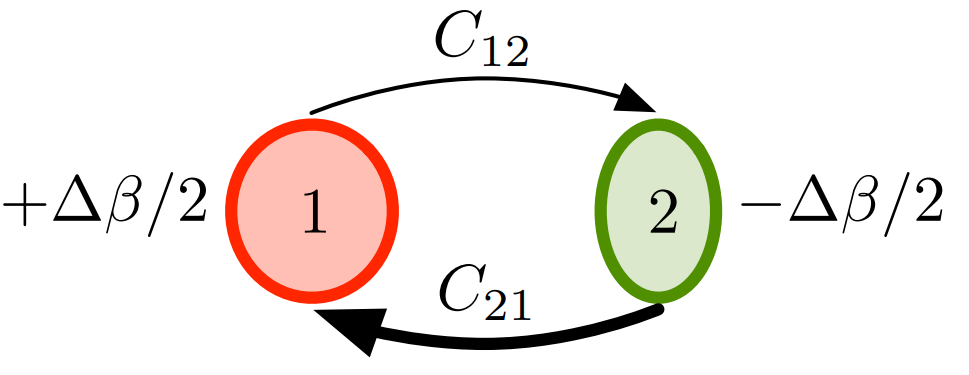
\includegraphics[width=0.4\linewidth]{media/nonsympaper}
	\caption{Schematic of non-symmetric coupling.}
\end{figure}
This \textit{non-symmetric} behavior can be quantified using the generalized non-orthogonal coupled-mode theory developed in Section~\ref{cap:CMTteo}, which includes the effect of modal overlap through the matrix \( \hat{P} \), encoding power normalization.

Considering a dimer composed of two non-identical waveguides, the dynamic equations for the modal amplitudes are written (see equation~(\ref{eqn:non-ortho-CMT-eqs})) as:
\begin{equation}
	-i
	\frac{d}{dz}
	\begin{pmatrix}
		P_{11} & P_{12} \\
		P_{12} & P_{22}
	\end{pmatrix}
	\begin{pmatrix}
		u_1 \\
		u_2
	\end{pmatrix}
	=
	\begin{pmatrix}
		H_{11} & H_{12} \\
		H_{12} & H_{22}
	\end{pmatrix}
	\begin{pmatrix}
		u_1 \\
		u_2
	\end{pmatrix}
	\iff
	-i\frac{d}{dz}\textbf{v} = \hat{H}' \textbf{v} \ ,
\end{equation}
where \( \textbf{v} = \hat{P}^{1/2} \textbf{u} \) represents an orthogonalized basis, and \( \hat{H}' = \hat{P}^{-1/2} \hat{H} \hat{P}^{-1/2} \) is the effective Hamiltonian in that basis. Since \( \hat{H} \) and \( \hat{P} \) are symmetric, \( \hat{H}' \) is also symmetric, which guarantees real eigenvalues. By proposing stationary solutions of the form \( \textbf{v}(z) \sim e^{i\lambda z} \), the generalized eigenvalue problem $\det(\hat{H} - \lambda \hat{P}) = 0$  is obtained.
It is important to emphasize that this orthogonalized basis \( \textbf{v} \) is not experimentally accessible: in a real setup, only modes localized in individual waveguides can be observed, which corresponds to the physical basis \( \textbf{u} \). Therefore, the experimental analysis of the dynamics must be performed in this basis, where the evolution is governed by the effective coupling matrix:
\begin{equation*}
	\hat{C} = \hat{P}^{-1} \hat{H} = \frac{1}{P_{11}P_{22} - P_{12}^2}
	\begin{pmatrix}
		P_{22}H_{11} - P_{12}H_{12} & P_{22}H_{12} - P_{12}H_{22} \\
		P_{11}H_{12} - P_{12}H_{11} & P_{11}H_{22} - P_{12}H_{12}
	\end{pmatrix}.
\end{equation*}
This system exhibits non-reciprocal dynamics: the energy transfer efficiency depends on the input channel. This asymmetry can be quantified experimentally through the \textit{intensity imbalance}, defined for each excitation \( i = L, R \) as:
\begin{equation*}
	I^i(z) \equiv \frac{P^i_1(z) - P^i_2(z)}{P^i_1(z) + P^i_2(z)} \ ,
\end{equation*}
and its absolute average as:
\begin{equation*}
	\bar{I}(z) \equiv \frac{|I^L(z) + I^R(z)|}{2} \ .
\end{equation*}
The quantity \( \bar{I}(z) \) is particularly useful for detecting global asymmetries in the dynamics: any deviation from zero implies a non-symmetric evolution, revealing the presence of non-reciprocal evanescent couplings.

\section{Numerical Validation}

Using the Eigenmode Expansion (EME) method (Section~\ref{cap:eme}), the dynamics of asymmetric dimers were simulated by injecting the same Gaussian initial condition in all cases. Figure~\ref{fig:nonotrho-num} shows the absolute average of intensity imbalances $\bar{I}(z)$ as a function of distance for $n_2 - n_1 = 1.75 \times 10^{-5}$ (weak asymmetry) and for $n_2 - n_1 = 5.00 \times 10^{-5}$ (strong asymmetry).

\begin{figure}[H]
	\centering
	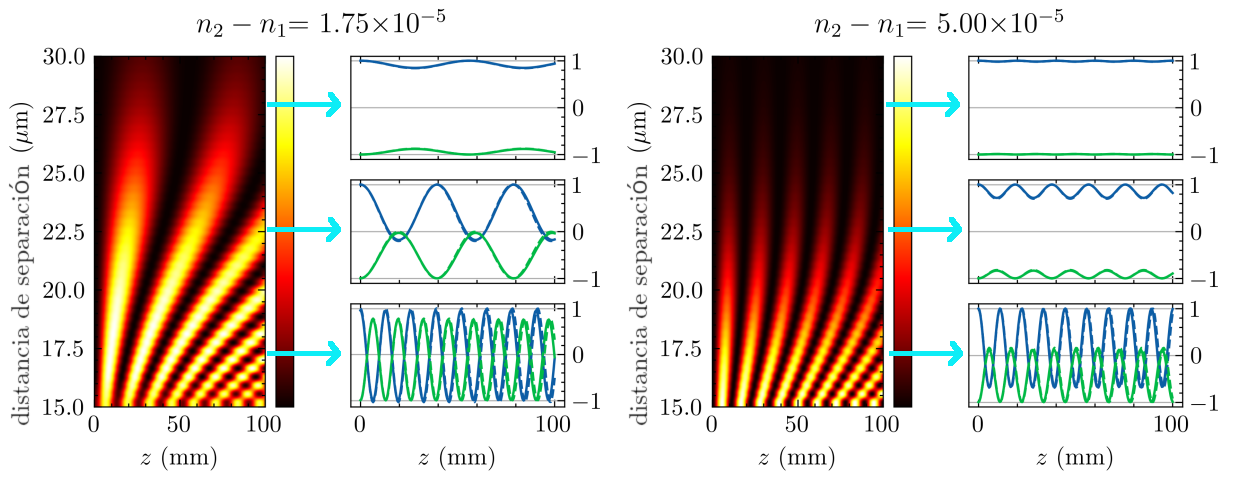
\includegraphics[width=\linewidth]{media/imbalance-nonortho.png}
	\caption[Absolute average of intensity imbalances $\bar{I}(z)$ as a function of propagation distance zz]{Absolute average of intensity imbalances $\bar{I}(z)$ as a function of propagation distance zz and the separation distance between waveguides, comparing two regimes: (1) weak asymmetry  ($\Delta n = 1.75 \times 10^{-5}$) and (2) strong asymmetry ($\Delta n = 5.00 \times 10^{-5}$). The values $I^L$ (green) and $I^R$ (blue) corresponding to three specific study cases are included.}
	\label{fig:nonotrho-num}
\end{figure}
\section{Experimental Verification}
To verify this effect, dimers were fabricated using the femtosecond laser writing technique described in Section \ref{cap:fs}, varying the input channel \( i \), the writing power \( P_{g}^i \), the distance between waveguides \( d \), and the effective propagation length \( z \). In particular, the case \( \Delta P = P_g^1 - P_g^2 = 5\,\mathrm{mW} \) was explored, with a separation  \( d = 18\,\mu\mathrm{m} \). Figure~\ref{fig:nosymexp} shows that excitation of the upper waveguide favors energy transfer to the lower waveguide, while the inverse excitation achieves a 1:1 energy distribution at $z\sim 11$ mm.
\begin{figure}[H]
	\centering
	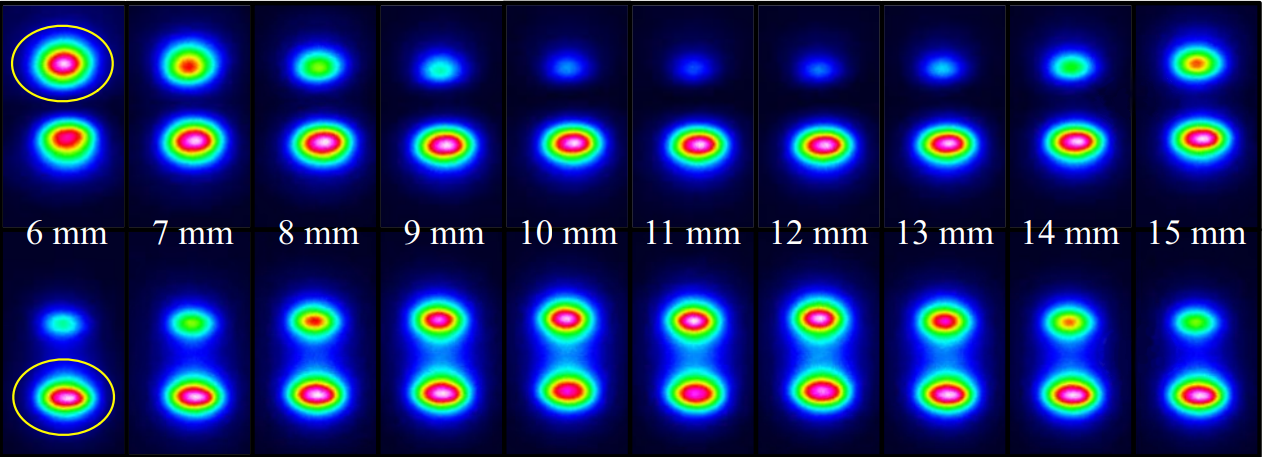
\includegraphics[width=0.9\linewidth]{media/nonsymm-exp.png}
	\caption[Output profiles for different propagation lengths.]{Output profiles for different propagation lengths  \( z_i \), exciting the upper waveguide (left) and lower waveguide (right), with \( d = 18\,\mu\mathrm{m} \). \label{fig:nosymexp}}
\end{figure} \vspace{-4ex} Using slab-type waveguides and TE modes (see Section \ref{cap:slab}), analytical expressions for the couplings are obtained:
\begin{equation*}
	\frac{C_{21}}{C_{12}} \approx \left( \frac{\Delta n_2}{\Delta n_1} \right)^2 e^{(\gamma_2 - \gamma_1) d}\approx \frac{P_2^1(z)}{P_1^2(z)} \ ,
\end{equation*}
where \( \gamma_i \) represents the evanescent decay coefficient of mode \( i \). his expression shows that the asymmetry increases with the separation between waveguides, with the difference between the modal decay rates $\gamma_2 - \gamma_1$ and with the square of the ratio of index contrasts $\Delta n_2/\Delta n_1$. 

\section{Implications and Applications}

This study demonstrates that non-symmetric coupling is a physical phenomenon that, in the absence of energy loss or gain, can be passively induced. Its implications include: \textit{breakdown of reciprocity}, without requiring magneto-optical materials or temporal modulation; \textit{modal asymmetry}, since the inequality between \( C_{ij} \) and \( C_{ji} \) affects the formation of symmetric/antisymmetric states and interference; \textit{directional optical devices}, such as asymmetric beam splitters or optical isolators; and its \textit{extension to lattices} with directed couplings. Together, these results allow for an extension of coupled-mode theory and open new opportunities in the design of optical lattices with directional functionality.